\documentclass[dvipsnames, svgnames, x11names]{beamer}

\usetheme{mytheme2024}
\usetikzlibrary{tikzmark}


\title{生物药剂学与药物动力学}
\subtitle{药物动力学的基本理论}
\author{张斌}
\institute[理工系]{河北农业大学 理工系}
\date{\the\year 年 \the\month 月}



\begin{document}

	
\maketitle


\begin{frame}
	\frametitle{学习目标}
	\begin{enumerate}
	  \item 熟悉药物动力学模型的概念以及药物在体内的速率过程 。
	  \item 掌握主要药物动力学参数的求算及其意义。
	\end{enumerate}
\end{frame}


\begin{frame}{}
	\begin{center}
		{\Huge \cbf{目 \ 录}}
	\end{center}
	\tableofcontents[subsectionstyle=hide/hide/show]
	\thispagestyle{empty}
	\addtocounter{framenumber}{-1}
\end{frame}


\section{药物体内转运的速率过程}


\begin{frame}
    \frametitle{药物体内转运速率}
	药物进入体内后 ， 随着血液循环被转运到机体各组织器官，最终在血液和组织之间达到动态转运平衡。体内不同部位的药物量或血药浓度随时间而发生变化 。 药物在体内转运的速率过程可借鉴化学反应动力学的方法进行描述 ， 即药物在体内某一部位的转运速率$\frac{\mathrm{d}X}{\mathrm{d}t}$与该部位药量$X$的关系符合下式 ：
	\[
		\frac{\mathrm{d}X}{\mathrm{d}t}=-kX^n
	\]
	在药物动力学研究中 ， 通常将药物体内转运的速率过程分为三种：
	\begin{enumerate}
	  \item 一级速率过程
	  \item 零级速率过程
	  \item 非线性速率过程
	\end{enumerate}
\end{frame}


\begin{frame}
	\frametitle{一级速率过程}
	一级速率过程：药物在体内某部位的转运速率与该部位的药量或浓度的一次方成正比
	\[
		\frac{\mathrm{d}X}{\mathrm{d}t}=-kX
	\]
    \begin{itemize}
      \item 一级速率过程也称为一级动力学过程、线性速率过程或线性药物动力学。
      \item 多数药物在体内的吸收 、 分布 、 代谢 、 排泄等动态变化过程都呈现一级速率过程 。
    \end{itemize}
	
	
	由于经典的药物动力学主要利用线性速率的原理 ， 将药物在体内的过程用线性微积分方程来描述 ，故经典的药物动力学也称为线性药动学。

	一级速率过程具有以下特点 ：
	\begin{enumerate}
	  \item 药物的生物半衰期与给药剂量无关 ；
	  \item 一次给药的血药浓度-时间曲线下面积与给药剂量成正比 ；
	  \item 一次给药情况下 ， 尿药排泄量与给药剂量成正比 。
	\end{enumerate}
\end{frame}


\begin{frame}
	\frametitle{零级速率过程}
	零级速度过程是指药物的转运速率在任何时间都是恒定的，与药物量或药物浓度无关。
	\[
		\frac{\mathrm{d}X}{\mathrm{d}t}=-k
	\]
	零级速率过程亦称零级动力学过程 。
	
	零级速率过程的药物，其生物半衰期随剂量的增加而延长；药物从体内消除的时间取决于剂量的大小 。
	\begin{blankblock}{}
		临床上恒速静脉滴注的给药速率以及控释制剂中药物的释放速率均为零级速率过程。
	\end{blankblock}
\end{frame}


\begin{frame}
	\frametitle{非线性速率过程}
	非线性速率过程的产生大多与给药剂量有关，因给药剂量不同而导致不同的药物动力学过程。
	\begin{itemize}
	  \item 当参与药物代谢的酶易被饱和或受到药物转运体数量限制时，有些药物在给药剂量较小(或血药浓度较低)时，药物体内的速率过程表现为一级速率过程；
	  \item 当给药剂量较大(或血药浓度较高)时，药物代谢酶被饱和或参与药物转运的载体被饱和，药物体内的速率过程表现为零级速率过程。
	\end{itemize}
	药物在体内的非线性速率过程可用米氏方程 （ Michaelis-Menten 方程 ） 进行描述 ， 因而也称 Michaelis-Menten 型速率过程或米氏动力学过程 。

	非线性速率过程的药物，半衰期与给药剂量有关 ， 血药浓度-时间曲线下面积与给药剂量不成正比。 
\end{frame}


\section{药物动力学模型}


\begin{frame}
	\frametitle{药物动力学模型}
	为了揭示药物在体内的动态变化规律性，常常要借助数学的方法来阐明体内药量随时间而变化的规律性，根据体内药量和时间的数据，建立一定的数学模型，求得相应的药动学参数，通过这些参数来描述药物体内过程的动态变化规律性。
	
	用数学方法模拟药物体内过程而建立的数学模型，称为药物动力学模型 ， 目前已建立的模型包括：
	\begin{itemize}
	  \item 房室模型
	  \item 基于统计矩原理的非房室模型
	  \item 非线性药动学模型
	  \item 生理药动学模型
	  \item 药动学和药效学结合模型
	  \item ……
	\end{itemize}
\end{frame}


\begin{frame}
	\frametitle{房室模型}
	房室模型是最经典的线性药物动力学模型。房室模型理论从速度论的角度出发，建立一个数学模型来模拟机体，它将整个机体视为一个由若干个房室组成的完整的系统，并将该系统按动力学特性划分为若干个房室，称之为房室模型。根据药物在体内的动力学特性，房室模型可分为单室模型、 双室模型和多室模型。
	
	\begin{itemize}
	  \item 房室只是数学模型中的一个抽象概念，并不代表解剖学上的任何一个组织或器官，因此房室模型的划分具有抽象性和主观随意性。
	  \item 只要体内某些部位药物转运的速率常数相同或相似 ， 不管这些部位的解剖位置与生理功能如何 ， 都可视为一个房室 。
	  \item 同一房室可由不同的器官 、 组织组成 ， 而同一器官的不同结构或组织 ， 可能分属不同的房室 。
	  \item 不同药物的房室模型及组成可能会不同 ；
	  \item 同一房室内各组织器官之间的药物浓度可以不同，各组织器官的药物处于动态平衡 。
	\end{itemize}
	  
\end{frame}


\begin{frame}
	\frametitle{单室模型}
	\begin{minipage}{0.58\linewidth}
		机体给药后药物立即分布至全身各体液和组织中 ， 并在体内迅速达到动态平衡 ， 此时整个机体可视为一个房室 （ 如图） ， 称为单室模型或一室模型 。

		\begin{alertblock}{应注意}
            符合单室模型的药物并不意味着机体各组织中的药物浓度在任何时刻都一样 ， 但是机体各组织中的药物浓度能随血药浓度的变化平行发生变化，即药物在机体各组织中的转运速率相同 。
        \end{alertblock}
	\end{minipage}\hfill
	\begin{minipage}{0.38\linewidth}
		\begin{center}
			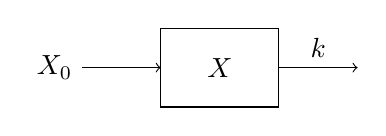
\begin{tikzpicture}
				\draw[->] (0,0) node[left]{$X_0$} --  (1,0);
				\draw (1,-0.5) rectangle (2.5,0.5) node[midway] {$X$};
				\draw[->] (2.5,0) -- (3.5,0) node[above,midway]{$k$};
			\end{tikzpicture}
		\end{center}
	\end{minipage}
\end{frame}


\begin{frame}
	\frametitle{双室模型}
	\begin{minipage}{0.58\linewidth}
		如图所示，机体给药后药物首先迅速分布于血流比较丰富的中央室，并且瞬间达到动态平衡 ， 然后再分布于血流不太丰富的外周室边室， 此类体内过程称为双室模型，又称二室模型 。    
		\begin{itemize}
		  \item 中央室可由心、肝、肾、肺等器官组成 。
		  \item 外周室可由皮肤、脂肪、肌肉、骨骼等组织组成 。
		  \item 药物只从中央室消除，药物在中央室与外周室之间能够可逆转运
		  \item 外周室中的药物与血液中的药物需经过一段时间方能达到动态平衡。
		\end{itemize}
	\end{minipage}\hfill
	\begin{minipage}{0.38\linewidth}
		\begin{center}
			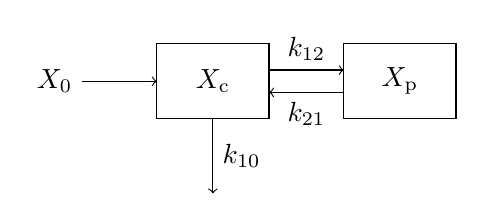
\begin{tikzpicture}[scale=0.95]
				\draw[->] (0,0) node[left]{$X_0$} --  (1,0);
				\draw (1,-0.5) rectangle (2.5,0.5) node[midway] {$X_\mathrm{c}$};
				\draw[->] (2.5,0.15) -- (3.5,0.15) node[above,midway]{$k_{12}$};
				\draw[->] (3.5,-0.15) -- (2.5,-0.15) node[below,midway]{$k_{21}$};
				\draw (3.5,-0.5) rectangle (5,0.5) node[midway] {$X_\mathrm{p}$};
				\draw[->] (1.75,-0.5) -- (1.75,-1.5) node[right,midway]{$k_{10}$};
			\end{tikzpicture}
		\end{center}
	\end{minipage}
\end{frame}


\begin{frame}
	\frametitle{多室模型}
	\begin{minipage}{0.58\linewidth}
		双室以上的模型称为多室模型 ， 它把机体看成由药物转运速率不同的多个单元组成的体系 。 
	\begin{itemize}
	  \item 多室模型的数学处理相当烦琐 ， 而单室模型和双室模型的数学处理相对较简单 ， 故多室模型不如单室模型和双室模型应用广泛 。
	  \item  从对药物体内过程理解的角度看 ，体内的房室数一般不宜多于 3 个 。
	\end{itemize}
	\end{minipage}\hfill
	\begin{minipage}{0.38\linewidth}
		\begin{center}
			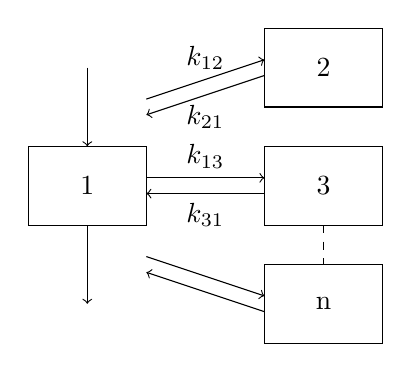
\begin{tikzpicture}
				\draw[->] (0.75,2) --  (0.75,1);
				\draw[->] (0.75,0) --  (0.75,-1);
				\draw (0,0) rectangle (1.5,1) node[midway] {1};
				\draw[->] (1.5,0.6) -- (3,0.6) node[above,midway]{$k_{13}$};
				\draw[->] (3,0.4) -- (1.5,0.4) node[below,midway]{$k_{31}$};
				\draw (3,0) rectangle (4.5,1) node[midway] {3};
				\draw (3,1.5) rectangle (4.5,2.5) node[midway] {2};
				\draw[->] (1.5,1.6) -- (3,2.1) node[above,midway]{$k_{12}$};
				\draw[->] (3,1.9) -- (1.5,1.4) node[below,midway]{$k_{21}$};
				\draw (3,-1.5) rectangle (4.5,-0.5) node[midway] {n};
				\draw[->] (1.5,-0.4) -- (3,-0.9);
				\draw[->] (3,-1.1) -- (1.5,-0.6);
				\draw[dashed] (3.75,0) -- (3.75,-0.5);
			\end{tikzpicture}
		\end{center}
	\end{minipage}
	
\end{frame}


\begin{frame}
	\frametitle{房室模型的局限性}
	\begin{enumerate}
	  \item 尽管经典房室模型在临床药动学研究中已得到广泛的应用 ， 但房室模型和机体的解剖结构 、 生理功能间没有直接联系 ， 只能通过血药浓度来推测靶器官的药物浓度 ， 而某些对组织具有高亲和力的药物如单克隆抗体药物 ， 或具有特异靶组织 、 靶器官效应的药物如靶向药物 ， 经典的房室模型无法客观表征作用部位的药物浓度 ， 致使药动学与药效学之间难以进行关联分析 。
	  \item 经典房室模型数据分析结果依赖于房室模型的选择 ， 而房室模型的选择带有一定的不确定性 。 同一种药物用不同的房室模型来解释 ， 相应的参数可能显著不同 。
	\end{enumerate}
\end{frame}


\begin{frame}
	\frametitle{生理药动学模型}
	生理药动学模型是一种整体模型 。 它是根据生理学 、 生物化学和解剖学的知识 ， 将机体的每个器官组织单独作为一个房室看待 ， 房室间的药物转运借助于血液循环连接并形成一个整体 。 药物在每一器官或组织（ 房室 ） 的分布和消除遵循物质平衡原理 。 
	\begin{itemize}
	  \item 生理药动学模型可描述任何器官或组织内药物浓度的经时变化 ， 可以提供药物体内分布的数据 ， 得到药物对靶器官作用的信息 ， 并可以模拟肝 、 肾功能 ， 提供药物体内生物转化的数据 ， 有利于阐明药物的作用机制 。
	  \item 各种哺乳动物的大多数生理参数 ， 如组织容积 、 血液流量等都是体重的函数 ， 以此为基础采用生理药动学模型 ， 可将不同种属的动物实验结果外推到人 ， 也
	  可将健康个体的实验结果外推到生理条件改变 （ 如血流速率 、 年龄 、 体重变化等 ） 或病理条件下（ 如肝 、 肾功能减退 ， 器官移植等 ） 的个体 ， 从而有利于药理学和毒理学研究结果的应用 。
	\end{itemize}
	
\end{frame}


\begin{frame}
	\frametitle{生理药动学模型的缺点}
	\begin{enumerate}
	  \item 模型结构复杂 ， 建立的数学方程求解困难 ， 限制了模型的推广和应用 ；
	  \item 建立模型时需要大量的动物生理参数 ， 增大了研究的工作量和难度 ；
	  \item 进行模型验证和调整时 ， 需要不同时间间隔的大量组织样本数据；
	  \item 生理药动学模型无法完全模拟机体生理条件 ， 尤其是在简化模型或降低计算难度的情况下 。
	\end{enumerate}
\end{frame}


\begin{frame}
	\frametitle{药动学和药效学结合模型}
	药动学和药效学结合模型（PK-PD模型）把药动学与药效学所描述的时间 、 药物浓度 、药物效应有机地结合在一起进行研究 。利用这一模型可以同时探讨机体对药物的作用 （PK） 及药物对机体的作用（PD）， 即明确药物浓度-时间-效应三者之间的相互关系 。
	
	根据药物作用方式和机制的不同 ， 完整 PK-PD 模型可分为四类 ：
	\begin{enumerate}
	  \item 直接连接与间接连接模型
	  \item 直接反应与间接反应模型
	  \item 软连接与硬连接模型
	  \item 时间依赖和时间非依赖模型
	\end{enumerate}
	对 PK-PD 研究一方面可为临床用药的安全性和有效性提供更为科学的理论依据 ； 另一方面则有助于阐明药物作用机制以及导致药效个体差异的因素 。
\end{frame}



\section{基本药物动力学参数}


\begin{frame}
	\frametitle{速率常数}
	速率常数是描述速率过程变化快慢的重要参数 。 一级速率常数以“时间” 的倒数为单位 ， 如min$^{-1}$或h$^{-1}$。 零级速率常数单位是 “ 浓度·时间$^{-1}$” 。
	
	速率常数有多种 ， 用于描述不同的药物转运过程 ， 常见的速率常数有 ：
	\begin{itemize}
	  \item[$k_\mathrm{a}$] 一级吸收速率常数
	  \item[$k$\ ] 一级总消除速率常数
	  \item[$k_\mathrm{e}$] 肾排泄速率常数
	  \item[$k_{12}$] 双室模型中 ，药物从中央室向周边室转运的一级速率常数
	  \item[$k_{21}$] 双室模型中 ， 药物从周边室向中央室转运的一级速率常数
	  \item[$k_{10}$] 双室模型中 ， 药物从中央室消除的一级消除速率常数
	  \item[$k_\mathrm{b}$] 生物转化速率常数
	\end{itemize}
\end{frame}


\begin{frame}
	\frametitle{速率常数}
	药物在体内的消除途径包括肾排泄 、 胆汁排泄 、 肺排泄 、 生物转化以及一切其他可能的途径 。 药物在体内的总消除速率常数$k$具有加和性 ，$k$为各个消除速率常数之和 ：
	\[
		k=k_{\mathrm{e}}+k_{\mathrm{b}}+k_{\mathrm{bi}}+k_{\mathrm{lu}}+\cdots 
	\]
	\vspace{-1em}
	\begin{itemize}
		\item[$k_\mathrm{e}$] 肾排泄速率常数
		\item[$k_\mathrm{b}$] 生物转化速率常数
		\item[$k_\mathrm{bi}$] 胆汁排泄速率常数
		\item[$k_\mathrm{lu}$] 肺消除速率常数
	  \end{itemize}
\end{frame}


\begin{frame}
	\frametitle{生物半衰期}
	\highlight{生物半衰期}是指药物在体内的量或血药浓度下降一半所需要的时间 ，以$t_{1/2}$表示 。 生物半衰期是衡量药物从体内消除快慢的指标。 因这一过程发生在生物体内（人或动物），且为了与放射性同位素的半衰期相区别，故称之为生物半衰期，这里统一简称为半衰期。
	\begin{itemize}
	  \item 一般来说 ， 代谢快 、 排泄快的药物 ， 其$t_{1/2}$短 ； 代谢慢 、 排泄慢的药物 ， 其$t_{1/2}$长 。
	  \item 对具有线性动力学特征的药物而言 ，$t_{1/2}$是药物的特征参数 ， 不因药物剂型或给药方法 （ 剂量 、 途径 ） 而改变 。
	  \item 同一药物用于不同患者时 ， 由于生理与病理情况不同 ，$t_{1/2}$可能发生变化 ， 故对于安全范围小的药物应根据患者病理生理情况制订个体化给药方案 。
	  \item 联合用药情况下 ， 可能产生药物相互作用而使药物$t_{1/2}$改变 ， 此时也应调整给药方案 。
	\end{itemize}
\end{frame}


\begin{frame}
    \frametitle{表观分布容积}
    表观分布容积 ($V$) ，是用来描述药物在体内分布的程度 ， 是表示全血或血浆中药物浓度与体内药量的比例关系 ， 其单位为 L 或 L/kg。通常用下式表示 ：
    \[
        V=\frac{X}{C}
    \]
    式中$X$表示体内药量 ； $C$表示相应的血药浓度 。它是指体内药物总量待平衡后，按测得的血浆药物浓度计算时所需的体液总容积（即理论上药物均匀分布所占有的体液容积）。

    当$V$已知时，可根据血浆浓度来推算体内外来化合物的总量。

    $V$虽然没有解剖学上的生理意义 ， 但是$V$值表示药物在血浆和组织间动态分布特性 ， 与药物的理化性质相关 。 
\end{frame}



\begin{frame}
	\frametitle{药峰时间($t_\mathrm{max}$)和药峰浓度($C_\mathrm{max}$)}
	药物经血管外给药吸收后出现的血药浓度最大值称为药峰浓度，达到药峰浓度所需的时间为药峰时间。与吸收速率常数相比它们能更直观和准确地反映出药物的吸收速率，因此更具有实际意义。药物的吸收速度快，则其峰浓度高，达峰时间短，反之亦然。
	\begin{figure}[htpb]
		\centering
		\setcounter{subfigure}{0}
		\subfloat[血管外给药的血药浓度-时间曲线]{
\includegraphics[height=4cm]{药峰时间}}\quad
		\subfloat[吸收速度A>B>C]{
\includegraphics[height=4cm]{药峰时间2}}
	\end{figure}
\end{frame}


\begin{frame}
	\frametitle{血药浓度-时间曲线下面积$AUC$}
	血药浓度-时间曲线下面积表示一段时间内药物在血浆中的相对累积量 。 面积越大，说明药物在血浆中的相对累积量越大。$AUC$常被用于评价药物的吸收程度。
	\begin{figure}[htpb]
		\centering
		
\includegraphics[width=.65\linewidth]{AUC}
	\end{figure}
\end{frame}

\begin{frame}
	\frametitle{生物利用度(bioavailability，$F$)}
	生物利用度是指药物经血管外给药后，药物被吸收进入血液循环的速度和程度的一种量度，它是评价药物吸收程度的重要指标。

	\highlight{绝对生物利用度}主要用于比较两种给药途径的吸收差异：
	\[
		F=\frac{{AUC_\mathrm{ext}}}{{AUC_\mathrm{iv}}} \times \frac{{D_\mathrm{iv}}}{{D_\mathrm{ext}}} \times 100\%
	\]
	式中$AUC_\mathrm{iv}$和$AUC_\mathrm{ext}$分别为静注给药和血管外给药后的血药曲线下面积，$D_\mathrm{iv}$和$D_\mathrm{ext}$分别为静注和血管外给药后的剂量。

	\highlight{相对生物利用度}主要用于比较两种制剂的吸收差异：
	\[
		F=\frac{{AUC_\mathrm{T}}}{{AUC_\mathrm{R}}} \times \frac{{D_\mathrm{R}}}{{D_\mathrm{T}}} \times 100\%
	\]
	式中$AUC_\mathrm{T}$和$AUC_\mathrm{R}$分别为服用受试制剂和参比制剂的血药曲线下面积，$D_\mathrm{T}$和$D_\mathrm{R}$分别为受试制剂和参比制剂的剂量。
\end{frame}


\begin{frame}
	\frametitle{清除率}
	清除率是指在单位时间内机体能将相当于多少体积血液中的药物完全清除 ， 即单位时间内从体内消除的药物的表观分布容积 。清除率常用“$Cl$”表示 。 整个机体的清除率称为体内总清除率(TBCL) 。 

	清除率的计算公式如下 ：
	\[
		Cl=\frac{-\mathrm{d}X/\mathrm{d}t}C=\frac{kX}C=kV
	\]
	\begin{itemize}
	  \item 清除率的单位用“体积/时间”表示 。
	  \item 清除率具有加和性 ， 体内总清除率等于药物经各个途径的清除率总和 。 
	  \item 多数药物主要以肝的生物转化和肾的排泄两种途径从体内消除 ， 因此药物在体内的总清除率等于肝清除率$Cl_\mathrm{h}$与肾清除率$Cl_\mathrm{r}$之和 。
	\end{itemize}
	
\end{frame}


\begin{frame}[t]
    \frametitle{}
    \begin{question}
        关于药物动力学参数表观分布容积（V）的说法正确的是
        \tcblower

        \only<1>{
            A. 表观分布容积是体内药量与血药浓度间的比例常数，单位通常是L或L/kg
        }
        \only<2>{
            \red{A. 表观分布容积是体内药量与血药浓度间的比例常数，单位通常是L或L/kg}
        }

        B. 特定患者的表观分布容积是一个常数，与服用药物无关

		C. 表观分布容积通常与体内血容量相关，血容量越大，表观分布容积就越大

		D. 特定药物的表观分布容积是一个常数，所以特定药物的常规临床剂量是固定的
        
    \end{question}
\end{frame}


\begin{frame}[t]
    \frametitle{}
    \begin{question}
        静脉注射某药，X0=30mg，若初始血药浓度为15μg/ml，其表观分布容积V为？
        \tcblower

        A. 20L

        B. 4L

		C. 30L

        \only<1>{
            D. 2L
        }
        \only<2>{
            \red{D. 2L}
        }
    \end{question}
\end{frame}


\begin{frame}[t]
    \frametitle{}
    \begin{question}
        某药静脉注射经3个半衰期后，其体内药量为原来的
        \tcblower

        A. 1/2

        B. 1/3

		C. 1/4

        \only<1>{
            D. 1/8
        }
        \only<2>{
            \red{D. 1/8}
        }
    \end{question}
\end{frame}


\begin{frame}[t]
    \frametitle{}
    \begin{question}
        对洛美沙星进行人体生物利用度研究，采用静脉注射与口服给药方式，给药剂量均为400mg，静脉给药和口服给药的AUC分别为40μg·h/ml和36μg·h/ml。基于上述信息分析，洛美沙星生物利用度计算正确的是
        \tcblower

        A. 相对生物利用度为55\%

        B. 绝对生物利用度为55\%

		C. 相对生物利用度为90\%

        \only<1>{
            D. 绝对生物利用度为90\%
        }
        \only<2>{
            \red{D. 绝对生物利用度为90\%}
        }
    \end{question}
\end{frame}










\end{document}